\chapter{国内外研究现状}

根据获取目标主机网络特征的方式,目前主机属性识别方法可分为主动方法和被动方法两类。因此,本章将从主被动两个角度分别介绍主机属性识别方法的技术思路和研究现状,然后针对目前该领域遇到的问题,明确本文的研究路线,最后对本章内容进行小结。

\section{主动识别方法}

主动识别方法通过构造特定的网络报文发往待测主机,根据待测主机的响应报文推断其主机属性,具有针对性强和准确性高等特点。然而,主动识别行为很容易被入侵检测系统或网络防火墙检测并阻止,经常导致目标主机无法收到探测数据包。因此,主动识别方法仅适用于少量场景。

\begin{figure}[!h]
    \centering
    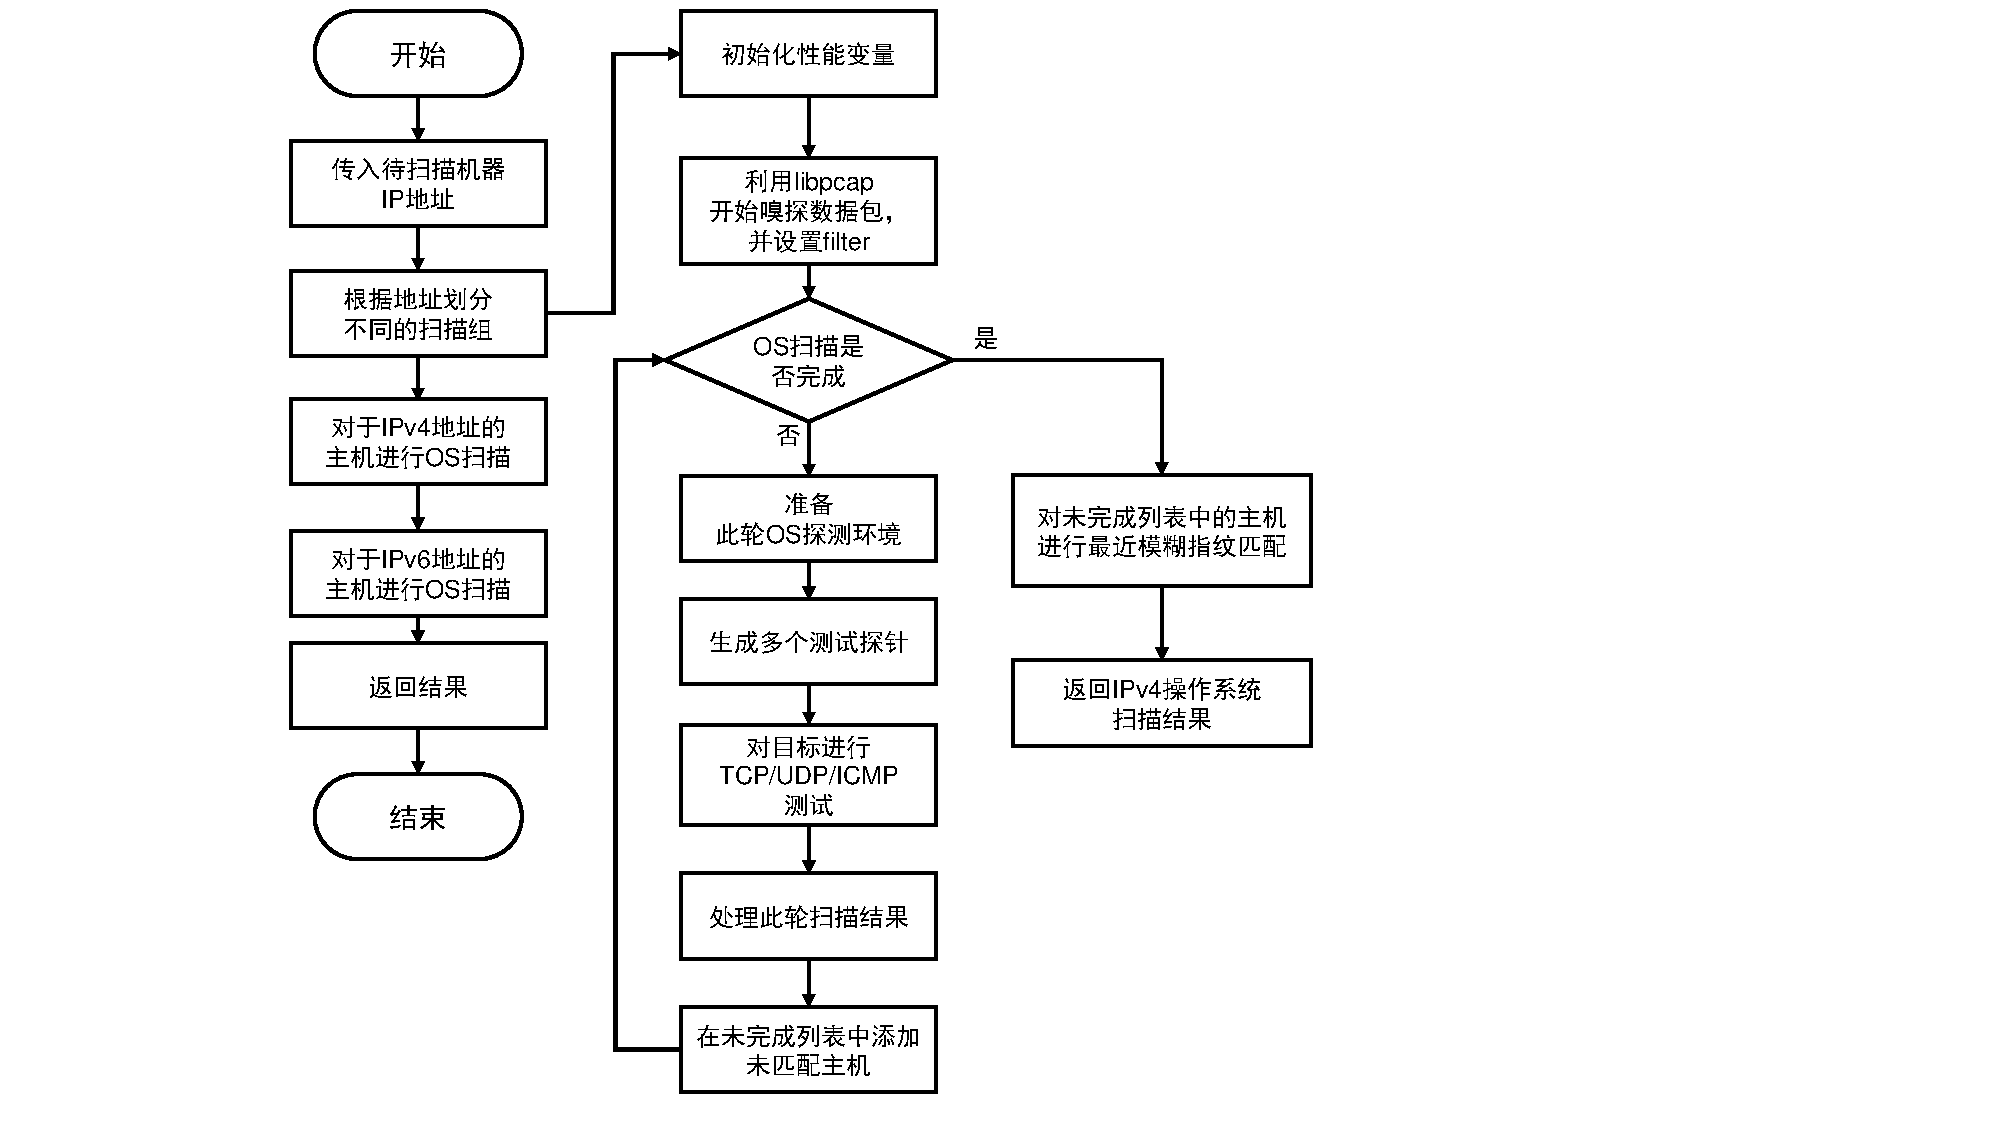
\includegraphics[width=0.7\textwidth]{nmap扫描}
    \bicaption{Nmap扫描流程图}{Nmap scanning flowchart}
\end{figure}

\citet{lyon1998remote}开发了著名的操作系统识别工具Nmap。Nmap工具扫描操作系统信息的流程如图2.1所示,其中网络探针包括6个用于获取序列折时间戳生成信息TCP探针,7个用于扫描开放端口的TCP探针、1个用于扫描关闭端口的UDP探针和2个ICMP探针,以此生成的指纹信息包括TCP时间戳、时钟频率、TCP标志、TCP可选项、IP字段等等。得到TCP/IP协议栈指纹后,Nmap工具会在一个已知系统的指纹数据库中进行匹配,从而获得待测指纹的操作系统信息。最新版本的Nmap同时支持对IPv6地址的主机进行操作系统扫描,其探测原理和IPv4网络中基本相同。该工具的缺点是易被入侵检测系统察觉,并且指纹库的升级需要消耗大量的人力成本。\citet{arkin2002remote}通过对比不同类型操作系统的ICMP协议栈实现,提出了一种基于ICMP报文探针的主动操作系统识别方法,通过向目标主机发送UDP和ICMP协议请求报文获取响应,然后解析响应报文格式得到目标主机的ICMP协议指纹,再借助模糊匹配方法从指纹库中推断目标主机的操作系统类型。该方法在当时解决了某些类型的操作系统因具备相同的TCP/IP协议栈指纹而无法识别的问题,有效提高了操作系统识别技术的准确率。

由于早期的主动操作系统指纹识别工具会向目标主机发送许多数据包,容易被网络防御设备检测,\citet{yarochkin2009xprobe2++}开发了Xprobe2工具,可以优先发送少量探针,降低被发现的可能性。该工具虽然具有模块编程接口,允许添加多种获取信息的网络探针,但默认建议只使用ICMP报文探针。Xprobe2对指纹库采取非严格匹配,对于指纹中的每个字段,分别根据匹配结果进行打分,并最终返回具有最高分数的匹配结果。此外,它还能发送一些针对程序应用层的测试探针。\citet{veysset2002new, beardsley2003snacktime, shamsi2014hershel}相继提出了仅利用单个SYN探针便可识别主机操作系统信息的方法。这些方法基于SYN包和ACK包重传差异,通过时间维度特征来扩展传统的指纹特征集。此类方法在发送探针后,都需要等到相对较长的时间(最多120秒),以便收集SYN包和ACK包重传后的时间差向量信息。

\citet{greenwald2007toward}提出了一种使用更少探针达到高精度识别操作系统的方法,仅需发送一到三个数据包便可获取远程主机的操作系统信息,其精度几乎与Nmap工具通过发送13个探针进行识别的方法一样高。并且他们还发现了TCP窗口大小和TCP可选项是携带特征信息最多的协议字段。同年,\citet{liuying2007ji}首次提出了仅依赖于TCP协议可选项字段的操作系统识别方法,识别原理是不同类型的操作系统对于网络探针的响应数据报文中的TCP可选项序列存在差异。虽然这种方式的探测成功率较高,但是识别的准确率较低。\citet{auffret2010sinfp}首次设计了一种基于IPv6网络进行操作系统识别的工具SinFP,并且此工具既可以进行主动识别,也可以进行被动识别。它首次配备了IPv6指纹库,如果待测指纹在IPv6指纹库中匹配失败,则可以回退到IPv4指纹库中再次进行匹配。为了实现IPv4指纹和IPv6指纹的自动转换,SinFP定义了以下对应关系:IPv4标志对应IPv6流标签,IPv4跳数对应IPv6跳数限制,IPv4分片标志对应IPv6流量类别等。由于操作系统通常在IPv4和IPv6之间共享TCP实现,因此这种转换是合理有效的。此外,SinFP利用启发式方法进行模糊匹配,可以解决部分未知指纹不能识别的问题。同样为了解决Nmap工具不能识别未知操作系统指纹的问题,\citet{zhoutiezheng2011ji}将支持向量机引入Nmap工具,但是该方法识别的操作系统类型范围较小,计算复杂度较高。

\section{被动识别方法}
被动识别技术利用网络监听技术获取目标主机与其他设备的镜像流量,通过从镜像流量中提取所需特征信息,结合数据库匹配方法或者机器学习算法,得到目标主机的属性信息,隐蔽性较强,但准确率相对主动方式较差。按照流量特征种类的不同,被动识别技术可以分为基于明文协议的方法,基于TCP/IP协议栈指纹的方法和基于流统计特征的方法。

\subsection{基于明文协议的方法}

由于早期协议开发未考虑数据安全的重要性,许多被广泛应用的网络协议都是明文协议。在未加密的HTTP协议、DNS协议、SSH协议等应用层协议中,都可以直接获取主机属性信息。例如,在Web应用HTTP流的GET请求报文中,首部的User-Agent字段通常都显式标注了客户端主机的属性信息,包括操作系统类型、版本以及浏览器类型。表2.1列出了部分主机属性与User-Agent字段的对应关系。此类方法的优势是识别速度非常快,准确率较高,但是随着流量加密技术的普及,基于明文信息的识别技术必将逐渐被淘汰。

\begin{table}[!htbp] 
    \bicaption{主机属性和User-Agent对应关系}{Correspondence between host attributes and User-Agent}
%    \label{tab:sample}
    \centering
    \footnotesize
    \setlength{\tabcolsep}{15pt}
    \renewcommand{\arraystretch}{1.2}
\begin{tabular}{cll}
\toprule
类型 & User-Agent字段 & 主机属性信息\\ \hline
\multirow{4}{*}{操作系统} & Windows NT 5.1 &Windows XP\\ 
& Windows NT 6.1 & Windows 7\\ 
& Windows NT 6.2 &Windows 8\\ 
& Windows NT 6.3 &Windows 8.1\\ \cline{2-3}
\multirow{4}{*}{浏览器} & Chrome/74.0.3729.169 & Chrome 74 \\
& OPR/43.0.2442.991 & Opera 43 \\
& Firefox/7.0.1 & Firefox 7 \\
& MSIE 6.0 & Internet Explorer 6 \\
\bottomrule
\end{tabular}
\end{table}

\citet{matsunaka2013passive}首次提出了一种基于DNS流量解析的操作系统识别方法。该方法主要利用各类操作系统的DNS查询特征不同进行识别,例如独特的查询域名,查询模式和时间间隔。虽然实验结果较好,但是该方法没有考虑异常查询行为的可能性。\citet{lastovicka2018passive}在一个大型校园网流量中对比了三种操作系统识别方法。结果表明,基于HTTP协议User-Agent字段的方法识别准确率最高,但识别范围仅能覆盖网络中一小部分主机。相反,基于TCP/IP协议参数的方法具有较广的识别范围,但识别精度较低。同时他们首次提出了一种新的基于特殊域名的识别方法,其性能不弱于前两种方法。此外,\citet{lastovicka2018passive}还测试了新型协议如IPv6和HTTP 2.0等对操作系统指纹识别技术的影响,认为基于HTTP协议User-Agent字段的方法和基于TCP/IP协议参数的方法在未来将不适用,只有基于特定域名的识别方法仍然可行。

\subsection{基于TCP/IP协议栈指纹的方法}

TCP/IP协议栈采用五层网络模型结构,主要包括物理层,数据链路层、网络层、传输层和应用层等。其中,网络层主要采用IP协议,IP协议可以提供无保证的尽可能快的网络传输服务,通过路由器将局域网连接成互联网。传输层主要采用TCP协议和UDP协议,TCP协议提供面向连接的服务,通过交互三次数据包完成连接的建立和相关参数的协商,如图2.2所示。

\begin{figure}[!h]
    \centering
    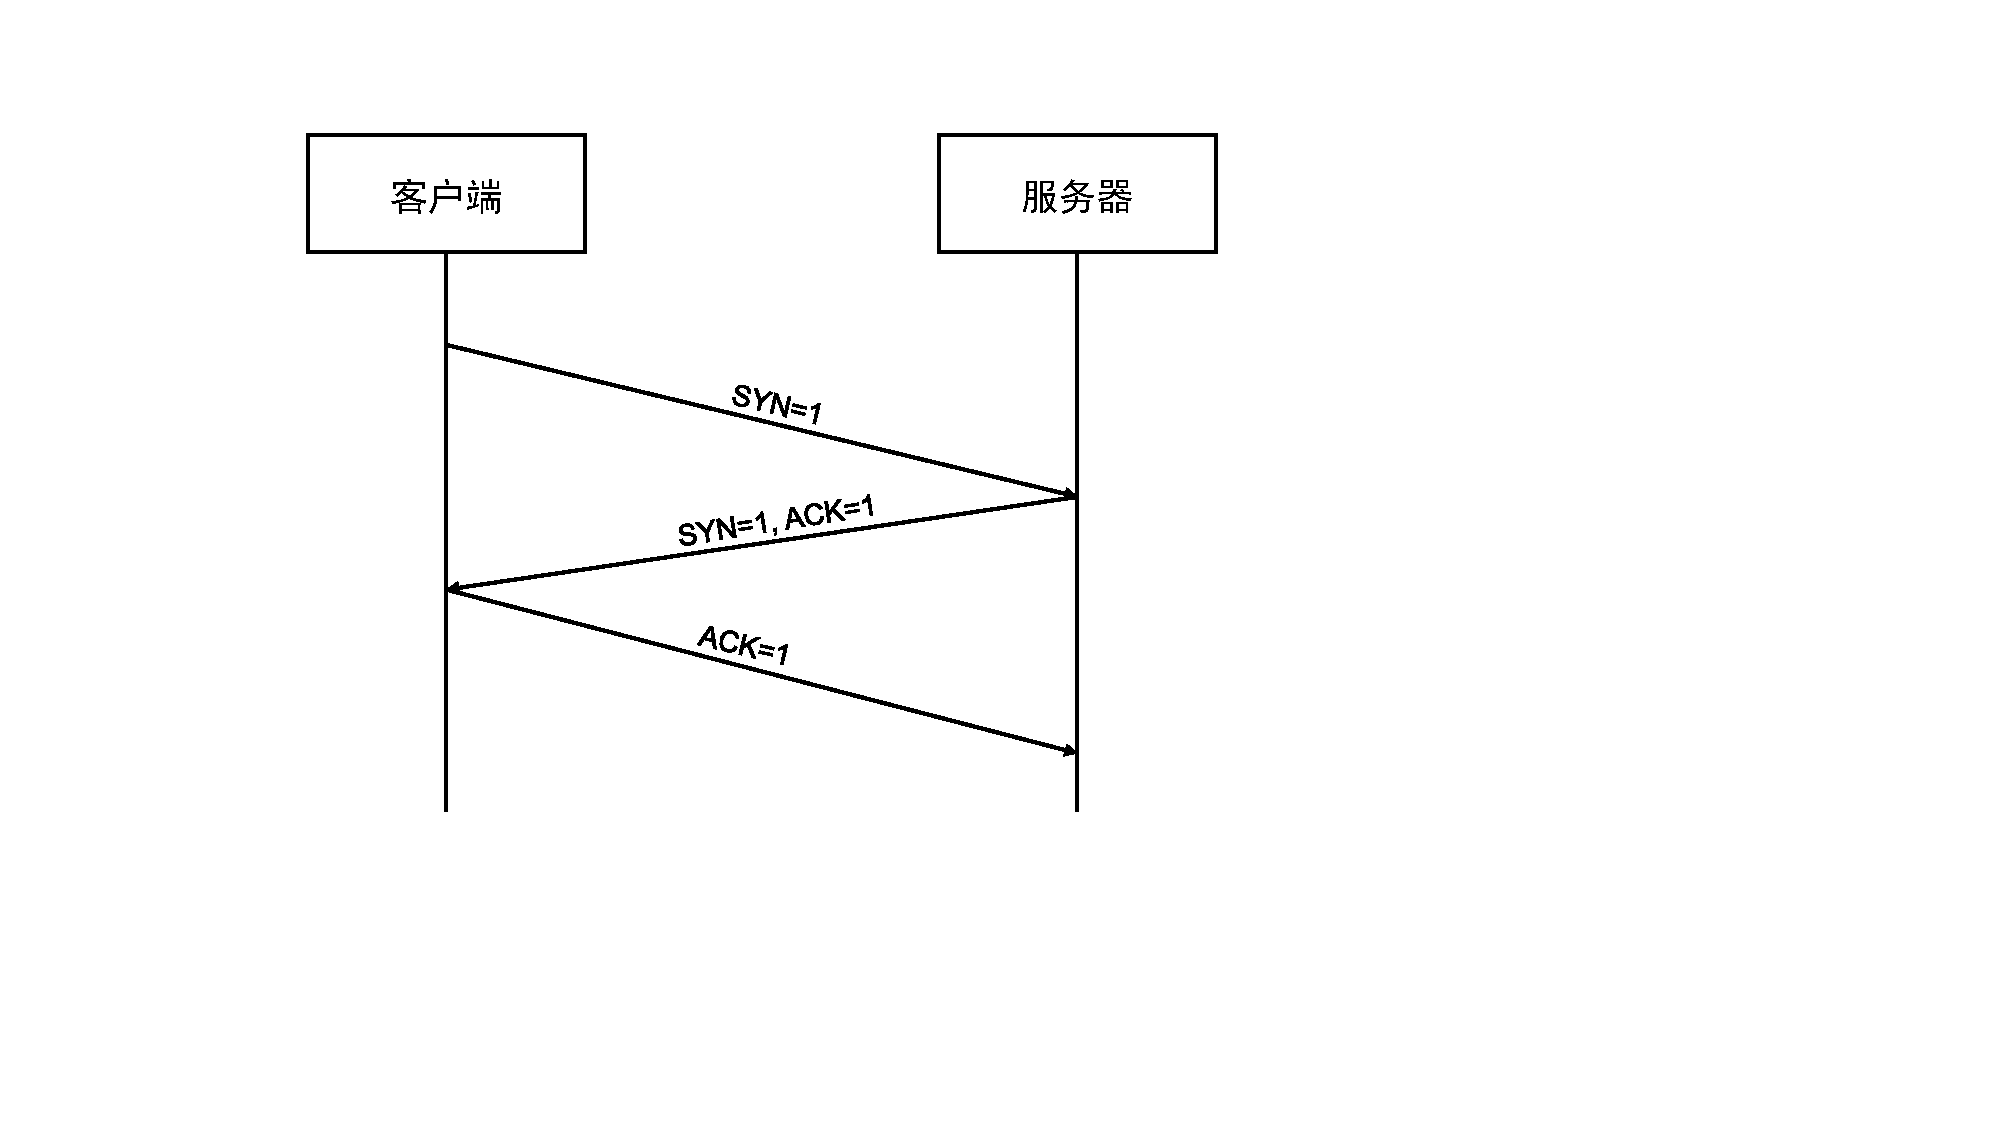
\includegraphics[width=0.5\textwidth]{TCP握手}
    \bicaption{TCP建立连接过程}{TCP connection establishment process}
\end{figure}

三个数据包的具体内容为:客户端首先向服务器发送一个请求建立连接的握手包,SYN字段标识为1,ACK字段标识为0,并附带客户端的协商参数,然后等待对方响应。若服务器正常运行,会回复一个SYN字段和ACK字段都标识为1的响应数据包,数据包附带服务器的协商参数。最后在协商完参数后,客户端会响应一个ACK标识为1的确认数据包,完成本次TCP连接。
 
由于不同属性的主机在实现TCP/IP协议栈时存在差别,称为TCP/IP协议栈指纹,可用于识别客户端的主机信息。TCP/IP协议栈指纹一般取自TCP建立连接过程中的第一个数据包,因为此数据包携带客户端主机的协商参数,如IP协议的分片标识、TCP协议的窗口大小和最大报文长度。表2.2列出了一些常见操作系统在以上参数的区别。

\begin{table}[!htbp] 
    \bicaption{常见操作系统TCP/IP协议栈指纹}{Common operating system TCP / IP protocol stack fingerprint}
    \centering
    \footnotesize
    \setlength{\tabcolsep}{10pt}
    \renewcommand{\arraystretch}{1.2}
\begin{tabular}{ccccc}
\toprule
操作系统 & IP跳数 & IP分片标识 & TCP窗口大小 & TCP最大报文长度\\ \hline
Windows 7 & 128 & 1 & 8192 & 1460 \\
Windows vista  & 64 & 0 & 8192 & 1200 \\
Linux 2.6 & 64& 1& 5792& 1460 \\
Linux 3.0 & 64 & 0 & 32736 & 1414 \\
MAC & 64 & 1& 33304 & 1460 \\
Openbsd & 64 & 1& 32768 & 1460 \\
\bottomrule
\end{tabular}
\end{table}

%TCP/IP协议栈指纹是基于不同属性主机在实现网络协议栈时的差异产生的,具有多样性和稳定性的特点。多样性是指不同属性的设备具备不同的协议栈指纹,稳定性是指同一类型的设备产生的指纹在一定的时期内不发生变化。

\citet{lippmann2003passive}实现了基于TCP/IP数据包头识别9种操作系统的分类器。该分类器主要利用KNN模型和决策树模型进行识别,通过交叉验证实验测试,准确率可以达到90\%。同时,\citet{beverly2004robust}借助概率学习思想,开发了一个朴素贝叶斯分类器,可以被动地从报文首部数据中推断出主机的操作系统类型,并比较了基于机器学习的方法和基于规则的推理工具(例如p0f的指纹数据库)之间的性能差异。最后通过分析一个因特网交换器上的流量,发现所有流量中的大部分流量都由一小部分操作系统产生。此外,作者利用该分类器统计了伪装在NAT设备后面的主机规模,并根据其他技术对结果进行评估,发现网络中由于NAT技术而导致的主机数量增多的比例大约为9\%。\citet{zalewski2006p0f}设计并开发了一套基于TCP/IP协议栈栈指纹的开源工具p0f,利用存储在文本文件中的指纹数据库来识别操作系统。\citet{barnes2013k}在p0f工具的基础上,开发出了k-p0f工具,其基于Linux内核实现,结合高效搜索算法,实现了高吞吐量、高精度的操作系统类型识别。\citet{richardson2010limits}讨论了操作系统指纹自动识别的局限性,提出了操作系统自动检测的四个主要挑战。第一个挑战是当前工具无法为不同的操作系统类型找到可概括样本空间并具有足够区分性的分类规则。其次,全自动工具无法有效利用协议的语义知识挖掘更多信息。最后两个挑战是全自动工具在实际网络中表现不好,并且普遍存在过拟合现象。总而言之,他们认为人工专家知识在未来一段时期内仍然是操作系统指纹生成技术中不可或缺的一部分。

在2014年,多篇关于主机属性识别技术的研究成果发表。\citet{chen2014fingerprinting}基于贝叶斯的规则分析比较了一系列TCP/IP协议首部特征对于操作系统分类任务中的有效性。结果表明,用于识别桌面端操作系统的一些技术并不能用于移动端操作系统的识别。\citet{jirsik2014identifying}提出了一种基于流的高性能操作系统检测系统,可以处理大规模流量。\citet{al2014improving}首次引入TCP FIN包特征,扩展了基于p0f指纹的特征集,可对移动端和桌面端的操作系统进行检测,并且检测的粒度更细。\citet{matouvsek2014towards}通过非监督机器学习中的聚类算法处理新的操作系统协议指纹,使得基于规则的推理方法具备了启发性。此外,还将指纹信息用于增强IPFIX标准记录,以便于大规模检测。

面对加密流量规模快速增长的现象,\citet{husak2016https}认为可以仅利用SSL/TLS握手参数便可识别客户端的主机属性。客户端在建立TLS连接时会发送一个Client Hello包,他们发现客户端在Client Hello包中存在主机标识。其中,最具有区分性的标识是客户端支持的密码套件列表。通过研究密码套件列表和HTTP协议的User-Agent字段之间的关系,提出可以构建密码套件列表和User-Agent信息的映射字典,基于该字典可以实时快速的识别客户端的主机属性,包括操作系统信息和浏览器信息。该研究的实验结果表明,此方法可以识别出95.4%的HTTPS网络流量。而在此之前,\citet{bujlow2015web}调查了当时已知的主机属性扫描技术,提出可以使用代理工具或者通过手动更改机器支持的密码套件列表等方法避免基于SSL/TLS协议指纹的恶意扫描活动。

\citet{tyagi2015packet}利用基于欧几里得距离的分类器可以从大约2000个SYN数据包中正确识别95.5%的数据包的操作系统。同时,\citet{fifield2015remote}通过查阅IPv6协议的的RFC文档,从中找出多处说明不详或未严格定义的协议实现,进而确定了基于IPv6协议字段的操作系统指纹,包括IPv6协议的长度字段,时间戳字段以及跳数限制字段等等。并利用线性分类器进行操作系统指纹的识别。\citet{anderson2017fingerprinting}的研究通过在一个时间窗口内聚合同一客户端发出的多条TLS会话特征,可以高精度地识别操作系统的主要版本和次要版本。\citet{aksoy2017operating}结合遗传思想,利用OneR模型、随机森林模型和J48模型三种机器学习算法对TCP/IP报文头部特征进行了最优特征子集选择。结果表明,遗传算法显著减少了需要分析的报文特征,同时也提高了识别性能。\citet{lavstovivcka2018machine}在计算效率、内存要求、准确率、精度和召回率等方面,比较了四种常用的机器学习方法性能,包括KNN模型,决策树模型,朴素贝叶斯模型和支持向量机模型等。实验结果表明,决策树模型是最适合处理主机属性发现任务的机器学习模型。

由于物联网近些年来得到了巨大的发展,同时继承了传统网络的安全性问题,操作系统识别引起了物联网网络安全性的研究关注。\citet{xuan2018identification}提出了一种基于RIPPER模型的被动操作系统识别方法。通过将其与现有的支持向量机和C45决策树分类算法进行实验对比。结果表明,基于RIPPER的算法具有更好的识别精度和识别效率。

\subsection{基于流统计特征的方法}

随着加密协议和私有协议的广泛应用,包括深度包检测技术在内的流量识别手段在越来越多的场景中失去作用,基于流统计特征的识别方法开始流行。流统计特征主要是指利用一次网络会话中所有数据包的包长、包达到时间以及包方向序列产生的统计值特征,例如最值、均值、均方差等等。此类方法一般需要结合机器学习模型或深度学习模型构建分类器,具有较高的识别准确率。

\citet{ruffing2016smartphone}认为移动设备产生的网络流量的时序特征由该移动设备运行的操作系统决定,提出通过分析网络报文时序的频谱以识别与操作系统相关的频率特性。由于无需利用报文内容,该方法可适用于流量加密的场景。通过收集运行 Android、iOS、Windows Phone和Symbian等操作系统的智能手机产生的流量,在观察时长为5分钟的报文序列后检测率能够达到90\%。然而该方法在判断同一操作系统的不同版本时效果并不理想。\citet{muehlstein2017analyzing}利用会话中每个数据包的长度序列特征和时间序列特征识别操作系统,结合以径向基函数作为内核的支持向量机模型,可以使得操作系统类型识别准确率达到96.06\%。

\section{本章小结}

本章主要从两个方面介绍了主机属性识别技术的研究现状。主动识别技术首先利用网络探针获取目标主机的响应报文,通过解析响应报文中的信息识别目标的主机属性。虽然具备准确率高和针对性强的优点,但易被网络防御设备干扰,适用场景有限。

而被动识别技术不需要和目标主机进行直接交互,只需监听网络中的数据包,通过提取并利用网络数据包中的协议首部信息、载荷信息和其他信息等便可识别目标主机属性。由于被动识别不受防火墙等安全设备的影响,其适用范围更广,缺陷是识别准确率相对较差。根据所需特征种类的不同,被动识别技术又分为基于明文协议的方法,基于TCP/IP协议栈指纹的方法和基于流统计特征的方法。每种方法的优缺点如表2.3所示。

\begin{table}[!htbp] 
    \bicaption{被动识别方法比较}{Comparison of passive identification methods}
%    \label{tab:sample}
    \centering
    \footnotesize
    \setlength{\tabcolsep}{15pt}
    \renewcommand{\arraystretch}{1.2}
\begin{tabular}{ccccc}
\toprule
被动识别方法 & 精度 & 性能 & 加密场景适用性 & 识别粒度\\ \hline
明文协议字段 & 高 & 快 & 否 & 细 \\ 
TCP/IP协议栈指纹 & 低 & 较快 & 是 & 细 \\ 
流统计特征 & 高 & 慢 & 是 & 粗 \\ 
\bottomrule
\end{tabular}
\end{table}

总体而言,当前主机属性识别领域依然存在以下问题:

\begin{itemize}

\item 识别成功率和准确率较低。由于入侵检测技术的日趋成熟,主动识别方法的适用范围越来越窄,成功探测到目标主机属性信息的成功率显著下降。所以未来应着重于研究被动识别方法,弥补其准确率较差的缺陷,从特征集和识别算法两个角度提升被动识别技术的效果和性能。

\item 识别粒度较粗,识别类型较少。大部分研究成果只能识别操作系统类型,无法识别操作系统版本和浏览器信息,而常见网络漏洞与操作系统类型和版本以及浏览器类型都密切相关,为了提高主机属性识别技术的应用价值,需要更细粒度和更广范围的识别方法研究。

\item 人工成本较高。无论是主动还是被动识别方法,主机网络指纹的设计都依赖于较高水平的专家经验,此外,在传统的指纹库匹配方法中,指纹库的更新也需要大量的人力和物力。因此,研究如何借助机器学习模型和表示学习方法识别主机属性具有重要意义。
\end{itemize}

面对上述挑战,本文将从被动角度面向加密网络进行主机属性发现技术的研究,综合当前主机属性识别方法的优点,扩展TCP/IP协议栈指纹,结合机器学习模型和神经网络模型,使得主机属性发现技术的准确率更高、性能更快、人工成本更低。

